%\begin{frame}{Opgave 4: Den adaptive metode}
%    Vi skal nu se på en anvendelse. Vi definerer en funktion ved
%\begin{align*}
%f(x) = 
%\begin{dcases}
%- \left( x - \sqrt{2} \right)^2 & x \leq \sqrt{2}\\
%\left( x - \sqrt{2} \right)^2 & x > \sqrt{2} \\
%\end{dcases}
%\end{align*} 
%    
%    Vi vil se på approksimation af integralet 
%    \begin{align}
%    \int_{0}^{3}f(x)dx    
%    \end{align}
%    % 
%\end{frame}

\begin{frame}{Approksimation af integralet}
\begin{align*}
f(x) = 
\begin{dcases}
- \left( x - \sqrt{2} \right)^2 & x \leq \sqrt{2}\\
\left( x - \sqrt{2} \right)^2 & x > \sqrt{2} \\
\end{dcases}
\end{align*} 
    
    Approksimation af integralet 
    \begin{align}
    \int_{0}^{3}f(x)dx    
    \end{align}
    % 
\end{frame}



\begin{frame}{Den adaptive metode}
    \begin{itemize}
        \item (a) Lav en Python funktion til beregning af funktionen defineret i (1).
        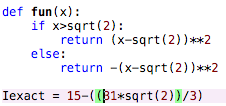
\includegraphics[]{images/1.4(a).png}
    \end{itemize}
\end{frame}


\begin{frame}{Den adaptive metode}
    \begin{itemize}
        \item (b) Vis, at den eksakte værdi af integralet er $15-\frac{31\sqrt{2}}{3}$.
        \item \begin{align*}
            \int^{\sqrt{2}}_0-(x-\sqrt{2})^2+\int^3_{\sqrt{2}}(x-\sqrt{2})^2=15-\frac{29\sqrt{2}}{3}-\frac{2\sqrt{2}}{3}= \\ 15-\frac{31\sqrt{2}}{3} 
            \end{align*} \\
            Ved at tage integralet for begge funktioner, og derefter plusse dem sammen, fås den eksakte værdi $15-\frac{31\sqrt{2}}{3}$ \\
    \end{itemize}
\end{frame}



\begin{frame}{Sammensat kvadratur}
\begin{align*}
\begin{array}{l|c|c|c}
\text{Metode} & \text{Resultat}& \text{Fejl} &  \text{Inddelinger} \\
\hline
\text{Midtpunkt}	& 3.8645984782 \cdot 10^{-01} & 7.662 \cdot 10^{-09}	& 4096 \\
\text{Trapez}		& 3.8645985304 \cdot 10^{-01} & 2.437 \cdot 10^{-09} & 8192 \\
\text{Simpsons}		& 3.8645985931 \cdot 10^{-01} & 3.833 \cdot 10^{-09} & 512 \\
\end{array}
\end{align*}
\end{frame}

\begin{frame}{Den adaptive metode}
    \begin{itemize}
%        \item (d) Lav i de tre tilfælde numeriske eksperimenter, baseret på fordobling af antal delepunkter, og brug dem til en eksperimentel bestemmelse af ordenen af de tre metoder. 
%       Stemmer resultaterne med teorien? Hvis der er afvigelser, hvordan kan
%        de så forklares?
        %Hvorfor springer orden så meget i Simpson efter 8192?
        \item 2. og 4. ordens - $O(h^2)$ $O(h^4)$
        \item Afrundingsfejl
        \item variationer i $f''$ og $f^{(4)}$
    \end{itemize}
    
$$\begin{array}{l|c|c}
\text{Metode} & \text{Inddelinger}& \text{Orden} \\
\hline
\text{Midtpunkt}	& 64		& 4 \\
\text{Trapez}		& 64		& 4 \\
\text{Simpsons}		& 4096	& 16 \\
\end{array}$$

$$\begin{array}{l|c|c}
\text{Metode} & \text{Inddelinger}& \text{Orden} \\
\hline
\text{Midtpunkt}	& 4		& 2 \\
\text{Trapez}		& 4		& 2 \\
\text{Simpsons}		& 16	& 4 \\
\end{array}$$

\end{frame}


\begin{frame}{Den adaptive metode}
    \begin{itemize}
%        \item (e) Prøv at anvende en simpel adaptiv metode til at bestemme integralet (2). 
%        Hvad sker der, hvis man inddeler i to delintervaller af samme længde. 
%        Hvordan bidrager de hver til fejlen i approksimationen? 
%        Angiv resultaterne for både trapezreglen og Simpsons regel.
        %Vi har svært ved at skulle dele i to delintervaller og alt det Python-fis
        \item For simpsons adaptiv: Integralet af funktionen fra $1.5$ til $3$ er præcist. 
        Derimod biddrager fra $0$ til $1.5$ til fejlen.
        \item For Trapez:  begge intervaller biddrager lige meget til fejlen - skyldes mindre grad af præcision.
    \end{itemize}
\end{frame}